%Centralizar verticalmente.
\newenvironment{midpage}{\vspace*{\fill}}{\vspace*{\fill}}
%Centralizar horizontalmente.
\newenvironment{midline}{\hspace*{\fill}}{\hspace*{\fill}}
\documentclass[12pts]{article}
\usepackage[utf8]{inputenc} 
\title{
	Prática de Eletrônica Digital 1 - (119466)
	\singlespacing
		Turma E (Unb - Gama)
	\singlespacing
	\begin{midpage}
	\begin {large}
		Relatório Experimento 2
		\singlespace
		Circuitos lógicos e combinacionais
	\end {large}
	\end{midpage}
}
\date{Agosto 26, 2016}
\usepackage{indentfirst}
\usepackage{setspace}
\usepackage{verbatim}
\usepackage[pdftex]{hyperref}
\usepackage{graphicx}
\begin{document}
\maketitle	
%\vspace{100 mm}
\begin{center}

\begin{tabular}{|c|l|r|}
\hline
Nome & Matrícula & Assinatura\\
\hline
Arthur Temporim & 140016759 & \\
\hline	
Eduardo Nunes & 140056189 & \\
\hline	
\end{tabular}

\end{center}


\newpage

\section{Sumário}

\begin{itemize}
	\item Introdução
	\singlespacing
	\item Experimentos
	\singlespacing
	\item Discussão
	\singlespacing
	\item Conclusões 
	\singlespacing
	\item Referências Bibliograficas
	\singlespacing
	%\item Diagramas esquemáticos
\end{itemize}

\newpage


\section{Introdução}
\iffalse
Introdução, indicando a delimitação do tema, apresentando a justificativa descrevendo o propósito do relatório.
\fi
	Neste relatório é apresentado os resultados dos três experimentos realizados na aula da prática da eletrônica digital 1.
	São apresentados no primeiro experimento a imagem do diagrama do circuito, o código VHDL e a saída. No segundo e no terceiro experimento, somente o código VHDL e a Saída. Todos os experimentos foram realizados utilizando a ferramenta \textit{Ise design suite}.

\section{Experimentos}
\iffalse
Parte Experimental, descrevendo os passos realizados, dificuldades e soluções para os problemas encontrados. Aqui, deve-se apresentar uma descrição dos resultados encontrados em forma de figuras, gráficos e tabelas.
\fi

\textbf{Experimento 01}
\singlespacing
	O primeiro experimento foi ampliar a quantidade de entradas do projeto 2 do pré relatório, ou seja, fazer um circuito comparador com 6 entradas. Foi primeiro desenvolvido o diagrama do circuito representado pela imagem abaixo e sua respectiva saída:

\begin{figure}[!htb]
  \centering
  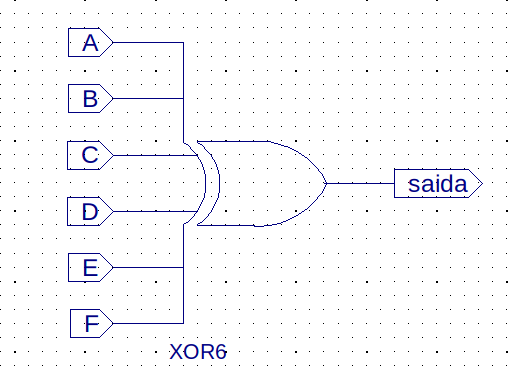
\includegraphics[scale=0.6]{img/diagrama01}
  \caption{Diagrama do circuito xor de 6 entradas - Ise Design Suite 14.7}
  \label{figRotulo}
\end{figure}

\begin{figure}[!htb]
  \centering
  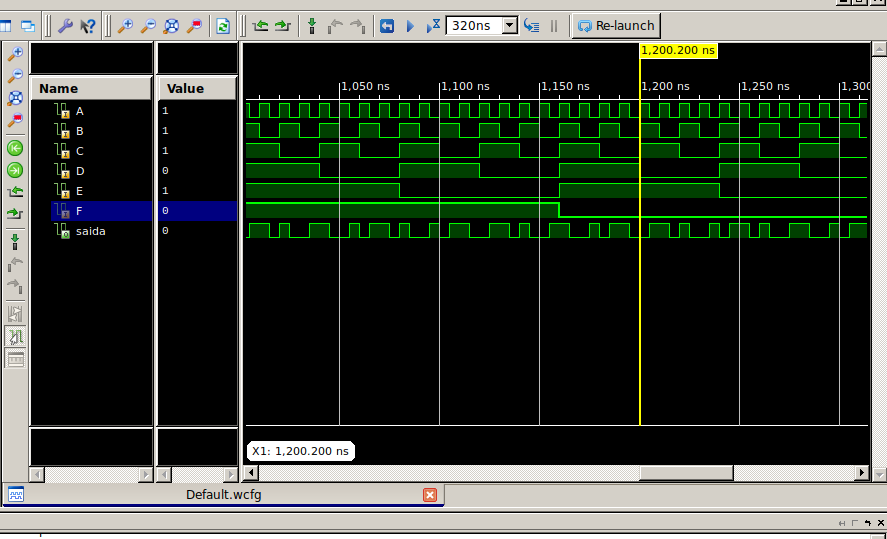
\includegraphics[scale=0.4]{img/saida01}
  \caption{Diagrama de ondas xor de 6 entradas - Ise Design Suite 14.7}
  \label{figRotulo}
\end{figure}
\newpage
Em logo, em seguida foi nos requisitado que fizemos o mesmo experimento só que usando agora o código em VHDL. Representado abaixo e sua respectiva saída:

\begin{figure}[!htb]
  \centering
  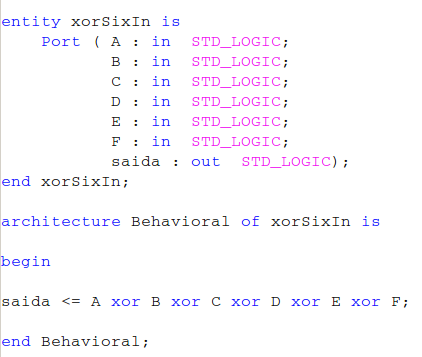
\includegraphics[scale=0.6]{img/vhdl01}
  \caption{Código VHDL xor de 6 entradas - Ise Design Suite 14.7}
  \label{figRotulo}
\end{figure}

\begin{figure}[!htb]
  \centering
  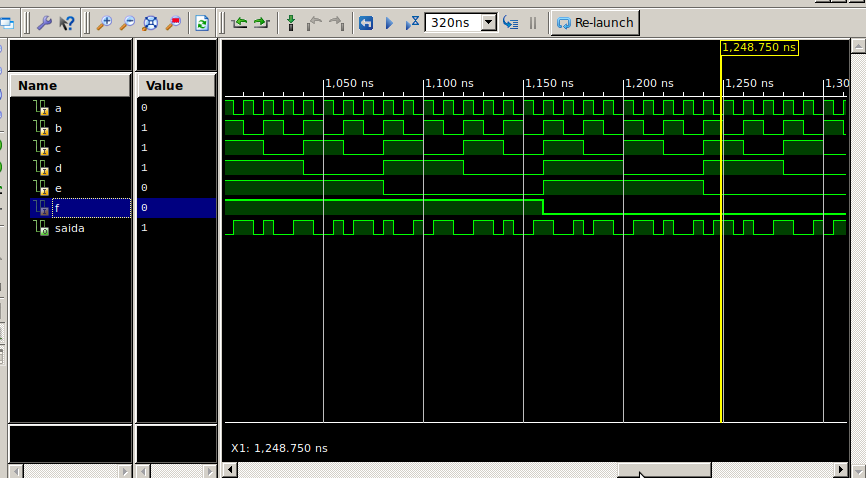
\includegraphics[scale=0.4]{img/svhdl01}
  \caption{Diagrama de ondas xor de 6 entradas - Ise Design Suite 14.7}
  \label{figRotulo}
\end{figure}

\textbf{Experimento 02}
\singlespacing
	O segundo experimento, tratava se de fazer um multiplexador de 2 entradas utilizando o VHDL e apresentar suas respectiva saída assim representado pelas imagens abaixo.

\begin{figure}[!htb]
  \centering
  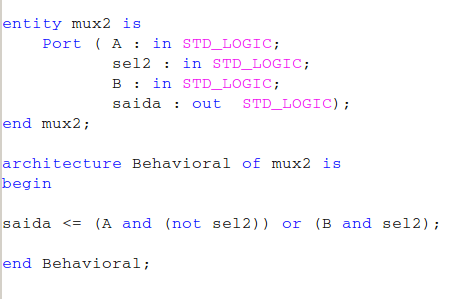
\includegraphics[scale=0.5]{img/vhdl02}
  \caption{Diagrama do circuito 01 - Ise Design Suite 14.7}
  \label{figRotulo}
\end{figure}

\begin{figure}[!htb]
  \centering
  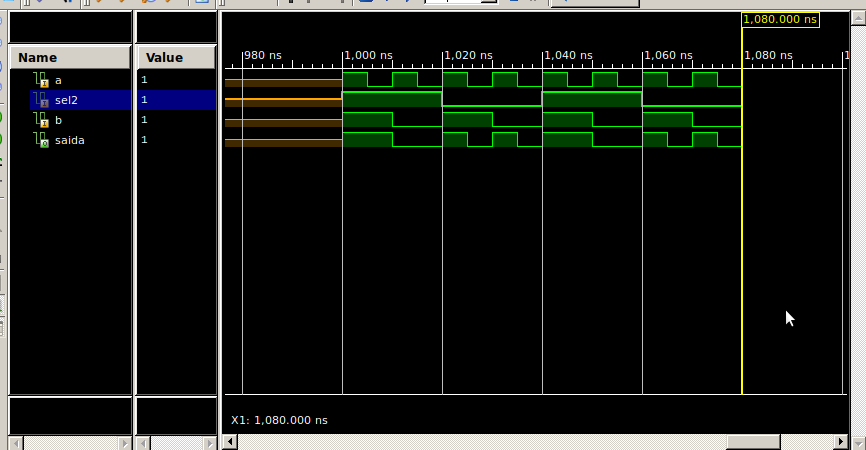
\includegraphics[scale=0.4]{img/mux2}
  \caption{Diagrama de ondas 01 - Ise Design Suite 14.7}
  \label{figRotulo}
\end{figure}

\newpage

\textbf{Experimento 03}
\singlespacing
	O terceiro experimento, tratava se de fazer um multiplexador de 4 entradas utilizando o VHDL e apresentar suas respectiva saída assim representado pelas imagens abaixo.

\begin{figure}[!htb]
  \centering
  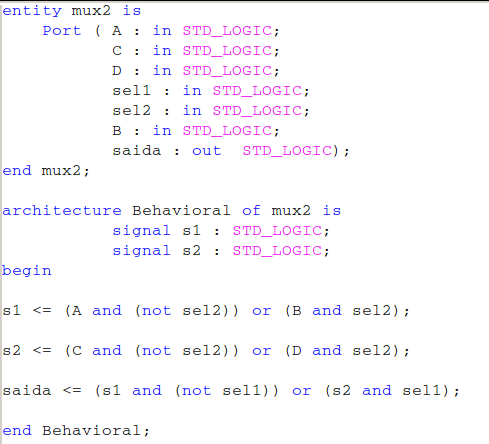
\includegraphics[scale=0.4]{img/vhdlmux4}
  \caption{Diagrama do circuito 01 - Ise Design Suite 14.7}
  \label{figRotulo}
\end{figure}

\begin{figure}[!htb]
  \centering
  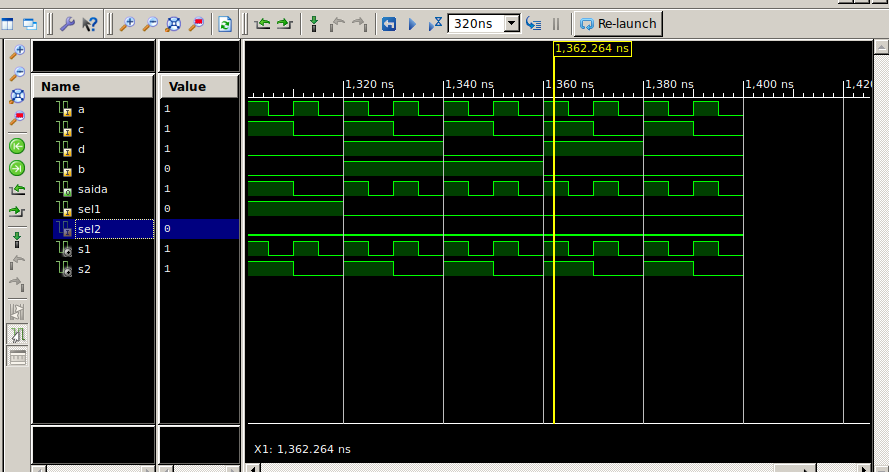
\includegraphics[scale=0.4]{img/mux4}
  \caption{Diagrama de ondas 01 - Ise Design Suite 14.7}
  \label{figRotulo}
\end{figure}




\newpage

\section{Discussão}
\iffalse
Discussão sobre os resultados encontrados, comentando detalhadamente as medições realizadas e dando a devida interpretação destas, informando se os objetivos da experimento foram alcançados. Esta é uma das partes mais importantes do relatório: aqui, há oportunidade para expressar os conhecimentos adquiridos na prática e fazer a interrelação com os fundamentos teóricos.
\fi

	Com a realização deste experimento foi possível adquirir a respeito de sistemas comparadores e multiplexadores assim como, aprender mais sobre a linguagem de descrição de hardware. O que por consequência gerou aprendizado da dupla e compreensão da implementação de circuitos.

\section{Conclusões}
\iffalse
Conclusões, mostrando os êxitos e eventuais problemas encontrados na realização do experimento, indicando as limitações, apresentando recomendações e/ou sugestões.
\fi

	Neste segundo relatório foi possível realizar todas as atividade com êxito sem dificuldades significativas tanto na implementação utilizando o software assim como em entender os circuitos.

\section{Referências Bibliográficas}
\iffalse
Referencias Bibliográficas, relacionadas e citadas de acordo com as normas da ABNT.
\fi
Prática de Eletrônica Digital I 2016.2 professores Henrique Marra Taira Menegaz,Leonardo Aguayo, Lourdes Mattos Brasil, Marcus Vinícius Chaffim Costa, Mariana Costa Bernardes Matias. UnB - FGA Agosto de 2015.

\iffalse
\section{Diagramas Esquemáticos}
Diagramas Esquemáticos. Todos os diagramas devem ser inseridos ao final do relatório em páginas separadas do texto, indicando a identificação do circuito, autor, revisor, versão e datas relevantes.
\fi
\newpage
\end{document}

%Exemplo de imagem
\iffalse
\begin{figure}[!htb]
  \centering
  \includegraphics[scale=0.3	]{nome_da_imagem}
  \caption{Descrição}
  \label{figRotulo}
\end{figure}
\fi

% Exemplo de tabela.
\iffalse
\begin{tabular}{|c|r|}
\hline
Material Utilizado & Quantidade\\
\hline
Cabo Banana-Banana & 2  \\
\hline
Fios de cobre & x \\
\hline
Cabo coaxial & 3  \\
\hline
CI 74HC00   & 1 \\
\hline
CI 74LS00   & 1 \\
\hline
Protoboard & 2 \\
\hline
Fonte de tensão MPL-3305M & 1 \\
\hline	
Multímetro Digital  & 1 \\
\hline
Gerador de funçoes iCEL modelo GV-2002 & 1 \\
\hline
Osciloscopio BK 2530 & 1 \\
\hline
\end{tabular}
\singlespacing
\fi
